\chapter[Detailed Cutting with Sparse Sampling]{Detailed Cutting of Thin Deformable Models with Sparse Sampling}
\label{chap:cutting}
\Lettrine{C}{ombining} interactive user actions and detailed convincing animations is crucial for user experience in simulation and games. Unfortunately, computational constraints limit the 
fidelity that can be achieved with physics-based animation
in interactive simulations. Often, the simulated objects lack detail compared to the rest of the virtual environment.
Furthermore, operations that modify the structure of the simulated objects, such as cutting, 
maybe incompatible with faster simulation methods.
When not prohibited, the latter generally exhibit strong limitations. Indeed, the level of sampling of a physically-based model usually depends on geometric complexity. Detailed cuts result in an increase of the sampling which directly impacts the performance. In practice, the number of samples is limited to ensure real-time performance. This limitation quickly prevents the user from applying detailed cuts.  
\paragraph*{}
In this chapter, we address the issue of enabling detailed cuts at interactive rates in  thin sheets of deformable material.
 Our method is able to capture detailed cuts while using a relatively low number of control nodes for the physically-based model.
Our approach to decoupling the sampling of the physical and of the geometric models, is to use a mesh-less simulation method called the frame-based model~\cite{Gilles2011} that we presented in Section~\ref{subsubsec:framebased}. In this method, the deformation field induced by animated frames is applied to the geometric model using skinning weights. As each frame can cover a large, detailed shaped region of the geometric mesh, only a few of them are typically required.
\paragraph*{}
To achieve user-driven cuts in a frame-based simulation, we allow cuts to be performed anywhere over the underlying mesh.
We build a non-manifold grid that keeps track of the mesh topology at the simulation level, and allows us to incrementally adapt the frames regions of influence in order to  represent the cut.
Although remaining low, the number of frame node does increase during a cut. 
In particular, when a model is cut apart, at least one frame is needed to represent each disconnected component. 
Therefore, we detect crucial cutting events, enabling us to automatically insert new frames when and where they are needed.
In order to reduce computations, we exploit the locality of the ongoing cutting gesture to incrementally update all the data used for the simulation.
\paragraph*{}
Our contributions includes:
\begin{itemize}
\item The building of a non-manifold grid to compute shape functions that faithfully represent the complex topology of the visual mesh while keeping a low number of control nodes (Section \ref{sec:adaptivesf}).
\item The dynamic re-sampling of new frames into disconnected parts (Section \ref{sec:resampling}).
\item The incremental update of the different components of the simulation that were concerned by the cut (Section \ref{sec:incremental}).
\end{itemize}

Our method can be used to simulate a wide variety of objects, such as stretchable cloth or pieces of paper. 
It features a very low number of frame nodes, high resolution mesh embedding, numerous and detailed cuts. 
Performance ranges from interactive to offline depending on the desired accuracy and complexity of the cuts.
We illustrate our method with examples inspired by the traditional Kirigami artform.
\paragraph*{}
We motivate our work with respect to existing methods for the simulation of cutting and fracture in Section~\ref{sec:starCutting}.
We choose to not include this section in Chapter~\ref{chap:star} for two reasons:
Firstly, this is a high level presentation of related works and we think a more detailed presentation of the underlying mathematics would be needed to be a part of the state of the art chapter;
Secondly, this configuration allows us to keep a more coherent discussion about our choices for the model.
In Section~\ref{sec:results}, we illustrate our method in different scenarios and detail the computational results. 
Finally, we discuss limitations and future work in Section~\ref{sec:cutting_conclusion}. 
\paragraph*{}
The works described in this chapter were presented at the conference \emph{MIG 2015}~\cite{Manteaux2015}.
A video illustrating the method and its results is available here: \url{https://youtu.be/coA_tcomWlE}.
%%%%%%%%%%%%%%%%%%%%%%%%%%%%%%%%%%%%%%%%%%%%%%%%%%%%%%%%%%%%%%%%
%                       RELATED WORK
%%%%%%%%%%%%%%%%%%%%%%%%%%%%%%%%%%%%%%%%%%%%%%%%%%%%%%%%%%%%%%%%
\section{Related work on cutting and fracture}
\label{sec:starCutting}

Cutting and fracture are both fascinating behaviors which can be simulated separately. 
In fracture, stress measurements predict how the material breaks. 
In cutting, the interaction with a tool define the cut path. 
For more details about cutting we refer the reader to the recent survey of Wu et al.~\cite{Wu2015}. 
Our review focuses on the modeling of topological changes in deformable models.

A first possibility consists in using the same model for physics simulation and visualization. Topological changes are then mostly modeled by remeshing operations. Simple and fast remeshing techniques such as element deletion or element splitting were proposed. The latter was used in the first simulation of brittle and ductile materials~\cite{OBrien1999},~\cite{OBrien2002}. 
 Methods that preserve element quality by local and global remeshing have also been developed. They recently lead to stunning results in the simulation of multi-layered paper tearing~\cite{Busaryev2013} and sheets tearing~\cite{Pfaff2014}. 
These methods cause the number of simulation nodes to vary over the course of a simulation, and this variation can be problematic in a realtime game context.  By limiting the
scope of remeshing predictable realtime performance can be achieved~\cite{Parker2009}.
An alternative to remeshing is to enrich elements with additional basis so that discontinuities can be represented. This is the core idea of the eXtended Finite Element Method (XFEM). It was successfully applied for offline cutting of discrete shells~\cite{Kaufmann2009}.

A second possibility is to separate the visual model from the physics model, this is known as embedding. Numerous embedding techniques have been proposed. The virtual node method~\cite{Molino2004} embeds ill-shaped elements that arise after remeshing inside of well-shaped elements. This allows to robustly simulate detailed cuts~\cite{Wang2014}. However, the number of nodes increases substantially with the complexity of the cut. To reduce it, hierarchical methods were proposed and real-time cutting in medical applications has been achieved using composite finite element method~\cite{Wu2011}. Still, the number of nodes grows quickly with the number of cuts and remains limited to ensure interactive frame rate. Meshless methods avoid the problem of element quality. However, boundary and discontinuities require extra effort to be sharply represented. \cite{Pauly2005} proposed to use visibility criterion to perform fracture. \cite{Steinemann2009} used the visual model as a visibility graph to define nodes connectivity. Both methods rely on a dense sampling near the surface of the model and quickly impact performances as the number  and the detail of cuts increases. There also have some work to carry complex materials~\cite{Nesme2009} and thin shells~\cite{Remillard2013} in hexahedra elements.

Embedding techniques have inspired our work. They allow interesting trade-off and show impressive cutting and fracture simulations. However, the relation between the resolution of the physical model and the visualization model remains very strong. Complex cuts result in a fast increase of the number of nodes. We want to reduce this connexion as much as possible. Complex topologies could be simulated with a very low number of nodes. Then, interactivity and intuitive control would be at hand.

Few models have been proposed that simulate detailed deformable objects using a low number of nodes. 
Subspace simulations~\cite{Barbic:2005:RTSI} compute a low basis of deformation modes in order to achieve real-time performance on detailed models. 
However, the low-basis is acquired after heavy precomputations. 
Interactive scenario could not handle the update of the basis at each topological change. 
More recently,~\cite{Gilles2011} and~\cite{Faure2011} proposed a physics-based skinning technique, called the frame-based method. 
Highly detailed meshes can be embedded in very coarse simulations. 
The control nodes are affine frames and the deformation field is described by a linear blend skinning. 
Classical continuum mechanics is then used to solve for the dynamics. 
Skinning weights, also called shape functions, are built on linear interpolation using discrete Voronoi regions. 
Thus, for each frame, they can represent a large region of influence with complex shape. 
Unfortunately, the current frame-based method does not allow the shape functions to reflect the topological changes of the embedded mesh.

\section{Overview of the method}

The goal of this work is to enable interactive detailed cutting of deformable thin sheets. 
The frame-based method exhibits some of the key features we are looking for: a very low number of nodes and a tunable separation between visual and physical models.  
We build on this framework and extend it to handle topological changes.

To transfer the cuts from the mesh to the frames, we continuously adapt the shape functions to the evolving mesh topology. 
This allows us to keep a constant number of nodes as long as there are no disconnected parts. 
In~\cite{Faure2011}, the shape functions are computed on a uniform grid.
The structure is simple and efficient. 
However, discontinuities that can be represented are very limited and strongly connected to the grid resolution. 
Instead, we build a non-manifold grid to compute topology-preserving shape functions (see Figure \ref{fig:spiralWeight}).

\begin{figure}[!h]
	\centering
	\begin{subfigure}[c]{0.18\linewidth}
		\centering
		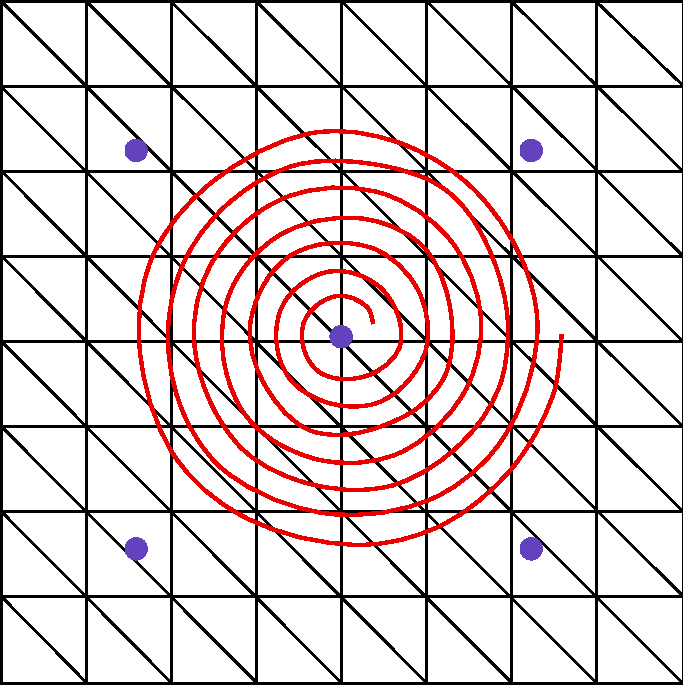
\includegraphics[width=\linewidth]{images/cutting-mig2015/spiral_mesh.pdf}
		\caption{\label{fig:spiralMesh}}
	\end{subfigure}
	\hspace{1.5cm}
	\begin{subfigure}[c]{0.68\linewidth}
		\centering
		
\includegraphics[width=\linewidth]{images/cutting-mig2015/sfRender_ff/weightShow.pdf}
		\caption{\label{fig:weightShow}}
	\end{subfigure}
	\caption[Frame-based cutting: Comparison of shape functions]{\label{fig:spiralWeight}
		Comparison between shape functions computed on a uniform grid and on a non-manifold grid. (a) The underlying mesh (black lines) is cut by spiral (red line) and sampled with five control frames (blue circle). (b) The shape functions for each of the frame with a uniform grid (top row) and with a non-manifold grid (bottom row). Values range from $1$ to $0$ and are respectively depicted from red to blue. We can observe that shape functions computed on the non-manifold grid strictly preserve the details and topology of the underlying mesh.}
\end{figure}

The main idea is that cut cells are duplicated and that each resulting instance stores different connectivities. 
Therefore, grid resolution depends much less on the mesh topology while keeping all topological informations.
We summarize our simulation loop in Algorithm~\ref{alg:simulationLoop} and detail our remeshing algorithm in appendix~\ref{appendix:remeshing}.

\begin{algorithm}[!h]
\caption[Frame-based cutting: Simulation loop]{\label{alg:simulationLoop}Simulation loop}
\begin{algorithmic}[0]
\For{each time step}
	\State perform a frame-based simulation step
	\State split the mesh along the cut
	\State embed the mesh in a non-manifold grid
	\State add new frames if required
	\State add new samples (collision, integration) if required
	\State compute shape functions on the grid
	\State incrementally update the samples
\EndFor
\end{algorithmic}
\end{algorithm}

\newpage

%%%%%%%%%%%%%%%%%%%%%%%%%%%%%%%%%%%%%%%%%%%%%%%%%%%%%%%%%%%%%%%%
%                      WEIGHT COMPUTATION / GRID
%%%%%%%%%%%%%%%%%%%%%%%%%%%%%%%%%%%%%%%%%%%%%%%%%%%%%%%%%%%%%%%%
\section{Adaptive shape functions} \label{sec:adaptivesf}

In this section, we first summarize how Voronoi shape functions are traditionally computed. 
Then we detail why a non-manifold grid is necessary, how to build it and how to use it to compute the shape functions on complex topology.

Let $w_{i}(x) : \Omega \rightarrow \mathbb{R}$ be the shape function for the $i$-th control frame, where $\Omega$ represents the domain. Starting from the Voronoi partition $V$ of the set of control frames, we can independently compute $w_{i}$ for each frame.

First, we compute the maximal distance $d_{max}$ from the control node to its Voronoi boundary $V_{b}$. Then we extend its Voronoi region $V_{i}$ to twice $d_{max}$. This gives a new region $V_{e}$ which describes the final boundary of the shape function. Now, we can compute $w_{i}$ inside $V_{e}$. We set $w_{i}$ to be $1$ at the frame position, $0$ at the others and $0.5$ on $V_{b}$. Finally, we linearly interpolate $w_{i}$ between $V_{b}$, the frame position and the boundary of $V_{e}$. We detail the interpolation in Algorithm~ \ref{alg:shapefunctioncomputation} and in Figure~ \ref{fig:shapefunctionconstruction}.

\begin{algorithm}[!h]
	\caption[Frame-based cutting: Shapefunction computation]{\label{alg:shapefunctioncomputation}Shapefunction computation}
	\begin{algorithmic}[1]
		\Procedure{Compute$\_$Shapefunction}{}
		\For{each frame $i$}
		\State $V_{i} \gets$ Voronoi region of $i$
		\State $V_{b} \gets$ boundary of $V_{i}$	
		\State $d_{max} \gets$ maximum distance to $V_{i}$ boundary
		\State $V_{e} \gets$ extend $V_{i}$ to $2.0 \times d_{max}$
		\LineComment{dist($A$,$B$) is the geodesic distance between $A$ and $B$}
		\For{each grid cell $j$ in $V_{e}$}
		\If{$j$ is inside $V_{i}$}
		\State $\displaystyle w_{i}(j) = 0.5\left(1 + \frac{dist(j,V_{b})}{dist(j,V_{b})+dist(j,i)}\right)$
		\ElsIf{$j$ is inside $V_{e}$}
		\State $\displaystyle w_{i}(j) = 0.5\left(1 - \frac{dist(j,V_{b})}{dist(j,i)-dist(j,V_{b})}\right)$
		\EndIf
		\EndFor
		\EndFor
		\EndProcedure
	\end{algorithmic}
\end{algorithm}

\begin{figure}[!h]
	\centering
	\begin{subfigure}[b]{0.20\linewidth}
		\centering
		
\includegraphics[width=\linewidth]{images/cutting-mig2015/buildSF_1.pdf}
		\caption{\label{fig:buildSF1}}
	\end{subfigure}
	\hspace{2cm}
	\begin{subfigure}[b]{0.20\linewidth}
		\centering
		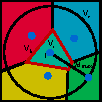
\includegraphics[width=\linewidth]{images/cutting-mig2015/buildSF_2.pdf}
		\caption{\label{fig:buildSF2}}
	\end{subfigure}
	\hspace{2cm}
	\begin{subfigure}[b]{0.20\linewidth}
		\centering
		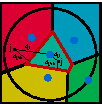
\includegraphics[width=\linewidth]{images/cutting-mig2015/buildSF_3.pdf}
		\caption{\label{fig:buildSF3}}
	\end{subfigure}
	\caption[Frame-based cutting: Voronoi shapefunction computation]{\label{fig:shapefunctionconstruction}
		Illustrations of Voronoi shape function computation. (a) Starting from samples (blue circles), we build a Voronoi diagram using Dijkstra's shortest path algorithm. (b) Then, for each frame and its region $V_{i}$, we compute the maximum distance $d_{max}$ to its Voronoi boundary $V_{b}$. We extend $V_{i}$ to twice $d_{max}$ which gives $V_{e}$. (c) Finally for each grid cell $j$ in $V_{e}$ we linearly interpolate using distance to the frame position and distance to $V_{b}$.}
\end{figure}

\subsection{Voronoi shape function}

In practice, the Voronoi diagram is computed using Dijkstra's shortest path algorithm on a grid in order to preserve geodesic distances. For each frame, the shape function is computed on the whole grid. As the grid resolution can be quite coarse, this is particularly fast. Negative values are clamped and weights are normalized to form a partition of unity. Then least-square approximation is performed to evaluate the shape function and its derivatives at specific positions.

Voronoi shape functions were designed in order to respect key properties that are particularly useful for physics-based animation~\cite{Faure2011} . First, they respect the Kronecker property, i.e $w_{i}(x) = \delta_{i}(x)$ where $w_{i}(x)$ is the shape function of node $i$, $x$ is a spatial position and $\delta_{i}$ is Dirac function. Second, they form a partition of unity, i.e $\sum_{i}w_{i}(x) = 1$. Third, they are built to be as linear as possible in order to produce uniform deformations. Finally, they can easily be biased by material properties in order to represent heterogeneous material.

%In the extension of the frame-based method~\cite{Faure2011}, they propose to use Voronoi shape functions. In this method, the region of influence of each frame is defined by an extension of its Voronoi region. Weights are linearly interpolated between the position of the frame and the boundary of the initial Voronoi region and they are extrapolated between the boundary of the initial Voronoi and the boundary of the extended Voronoi. In their paper, the Voronoi diagrams are computed on a discrete grid with a 8 neighbor connectivity using a Dijkstra algorithm. Weights and weight derivatives are then interpolated to specific sample positions such as mesh vertices or integration points or collision points. Weights are ensured to be linear along shortest path. This method allows to bias the distance computation by a material map in order to build weights that can represent heterogeneous material. In our method we use the same shape functions in order to represent large regions and heterogeneous materials. However we need to adapt the shape functions along the simulation to take into accounts the cuts.
%Shape functions describe the influence region of each node. In linear finite element methods, this region is clearly delimited by the elements that surrounds each vertex. Thus topology is naturally represented by the mesh itself. In mesh-less methods, 
%Each vertex influence 
%barycentric linear shape functions are used in triangular and tetrahedral meshes. They naturally represent the topology of the mesh and produce uniform deformations. In mesh-less methods, each node 
%The design of shape functions for skinning deformation is an active topic of research. Several key features have been identified in order to produce plausible deformations.
%Three key features that ensure plausible deformations have been identified. The first one is that the shape function should decrease with respect to the distance from the corresponding control node. The second one is that it should be as linear as possible in order to produce uniform deformations. Finally, it should respect the Kronecker property in order to provide easy  manipulations.
%Usually, three key features should be preser
%They should  Generally, the function decreases from $1$ to $0$ from the node position 
%Linear shape functions ensure that the material deform uniformly with the frame motions. 
%Usually, we want the region attached to a node to deform uniformly with it. Therefore we use linear weights
%the region of influence of each control frame
%The design of skinning weights is an active topic of research.
%Skinning weights describe the region of influence of the control frames and the type of influence. Generally we want the space to deform uniformly with the frames and so we use linear weights. When the region of a node is a simple shape such as a set of triangles or a quads, one can use well known weights such as barycentric or bilinear weights. However, when we do not want to describe the deformation field using a specific geometry, it is much more challenging to design shape functions. Most of the meshless methods use overlapping spline kernel with local support to describe the deformation field. Unfortunately this requires relatively dense sampling to cover the whole region. Nevertheless, both methods use local shape functions and assume that the number of nodes is important. In procedural animation, design of skinning weights is an active topic of research. The goal is to design weight that can cover regions of different sizes, while respecting the topology in order to provide intuitive control of a shape. An important step was achieved by the work of~\cite{Joshi2007} where they propose to use harmonic coordinates. Those skinning weights provide control over large regions while keeping the coherency of the topology. Unfortunately, those weights are highly nonlinear and results in unconvincing behavior in physics-based simulation. 

\subsection{Non-manifold grid}

As mentioned above, in~\cite{Faure2011}, shape functions are computed on a uniform grid using Dijkstra's shortest path algorithm to compute geodesic distance. Starting from a uniform grid with a 8-neighbor connectivity, we could reflect topological change by changing the connectivity of the cut cells. Then, when we re-compute shape functions, the topology would automatically be taken into account as we use geodesic distance. 

Unfortunately, this strategy is very limited for uniform grid and would only work in simple cases. For instance, several cuts that intersect or that create disconnected components inside one cell could not be represented. Even without cut, small gaps that lie inside one cell could not be correctly represented. Geodesic distances would be false and the object would behave as if there were no cuts or gaps. Augmenting the resolution would not solve the problem. We would fight the same issue as previous methods. Our grid resolution would be highly dependent on the complexity of the topology and the geometry of the object. It would directly impact performances.

We want each grid cell to be able to represent  the connectivities of the different disconnected components that lie in the cell. To do so, each cut cell is duplicated as many times as it contains disconnected parts. Each duplicate has a specific connectivity built from the material connectivity. This results in a data structure called \emph{non-manifold grid} (see Figure \ref{fig:nonmanifoldgridillustration}).

\begin{figure}[!h]
	\centering
	\begin{subfigure}[b]{0.20\linewidth}
		\centering
		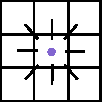
\includegraphics[width=\linewidth]{images/cutting-mig2015/connectivity.pdf}
		\caption{\label{fig:connectivity}}
	\end{subfigure}
	\hfill
	\begin{subfigure}[b]{0.30\linewidth}
		\centering
		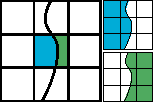
\includegraphics[width=\linewidth]{images/cutting-mig2015/simple_cut.pdf}
		\caption{\label{fig:simplecut}}
	\end{subfigure}
	\hfill
	\begin{subfigure}[b]{0.40\linewidth}
		\centering
		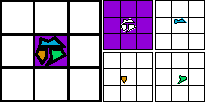
\includegraphics[width=\linewidth]{images/cutting-mig2015/little_pieces.pdf}
		\caption{\label{fig:littlePieces}}
	\end{subfigure}
	%\hfill
	%\begin{subfigure}[b]{0.24\linewidth}
	%\centering
	%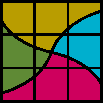
\includegraphics[width=\linewidth]{images/cutting-mig2015/multi_cut.pdf}
	%\caption{\label{fig:multicut}}
	%\end{subfigure}
	\caption[Frame-based cutting: Non-manifold grid illustration]{\label{fig:nonmanifoldgridillustration}
		Illustrations of different possibilities for a non-manifold cell with eight connectivity (a). In (b), the cell is simply cut into two cells. Each duplicate of the cut cell has a specific connectivity that represent the cut topology. In (c), multiple disconnected components can be contained inside one cell. The cell is duplicated four times. Three of the duplicates have no connectivity. However they can embed complex geometry and then be simulated by adding new frames for each of the component. The fourth duplicate keeps its eight neighbors and remains independent from the three other.}
\end{figure}

Non-manifold grids are used by many other cutting methods to embed fine geometric details in coarse finite element simulations. However, we make a completely different use of it. Instead of duplicating control nodes as the cells are cut, thereby increasing their number and the computation time, we use the grid to adapt the shape functions to the evolving topology of the mesh. Most of the time, the number of nodes can remain constant while representing detailed geometry and multiple cuts.

\newpage 

There are several ways to compute this non-manifold grid. In our method, we start by embedding the mesh in a uniform grid. Mesh elements that overlap a grid cell are detected using intersections tests and are assigned to it. Then, for each grid cell, we use a flood fill algorithm to detect the disconnected parts of the mesh. This informs about how many duplicates need to be created for the cell. Finally, for each duplicate we establish its connectivity by comparing its geometry with the geometry of the neighbor cells duplicates. We summarize our method in Algorithm~\ref{alg:nonmanifoldbuilding} and illustrate the main steps in Figure~\ref{fig:nonmanifoldgridbuilding}.

\begin{figure}[!h]
	\centering
	\begin{subfigure}[b]{0.20\linewidth}
		\centering
		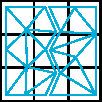
\includegraphics[width=\linewidth]{images/cutting-mig2015/buildNMG_1.pdf}
		\caption{\label{fig:buildNMG1}}
	\end{subfigure}
	\hfill
	\begin{subfigure}[b]{0.20\linewidth}
		\centering
		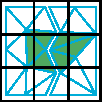
\includegraphics[width=\linewidth]{images/cutting-mig2015/buildNMG_2.pdf}
		\caption{\label{fig:buildNMG2}}
	\end{subfigure}
	\hfill
	\begin{subfigure}[b]{0.20\linewidth}
		\centering
		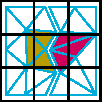
\includegraphics[width=\linewidth]{images/cutting-mig2015/buildNMG_3.pdf}
		\caption{\label{fig:buildNMG3}}
	\end{subfigure}
	\hfill
	\begin{subfigure}[b]{0.20\linewidth}
		\centering
		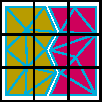
\includegraphics[width=\linewidth]{images/cutting-mig2015/buildNMG_4.pdf}
		\caption{\label{fig:buildNMG4}}
	\end{subfigure}
	\caption[Frame-based cutting: Non-manifold grid building]{\label{fig:nonmanifoldgridbuilding}
		We describe the building of the non-manifold grid for the center cell of the grid. (a) The mesh is embedded in a uniform grid. (b) First, we store the overlapping geometry in the cell. (c) Then we detect disconnected parts using a flood fill algorithm. (d) Finally the cell is duplicated. For each duplicate, we look for other duplicates that share geometry and establish its connectivity.}
\end{figure}

\newpage

\begin{algorithm}[!h]
\caption[Frame-based cutting: Non-manifold grid building]{\label{alg:nonmanifoldbuilding}Non-manifold grid building}
\begin{algorithmic}[1]
\Procedure{Build$\_$Non$\_$Manifold$\_$Grid}{grid $G$, mesh $M$}
\State \textsc{Build$\_$Grid$\_$Geometry}($G$,$M$)
\State \textsc{Duplicate$\_$Grid$\_$Cell}($G$)
\State \textsc{Build$\_$Grid$\_$Connectivity}($G$)
\EndProcedure
\State
\Procedure{Build$\_$Grid$\_$Geometry}{grid $G$, mesh $M$}
\For{each cell $i$ of $G$}
\State Store overlapping element of $M$
\EndFor
\EndProcedure
\State
\Procedure{Duplicate$\_$Grid$\_$Cell}{grid $G$, mesh $M$}
\For{each cell $i$ of $G$}
\State $C \gets $ disconnected component of $M$ in $i$
\For{each component j of $C$}
	\State Duplicate the cell $i$
	\State Store $j$ in the duplicate
\EndFor
\EndFor
\EndProcedure
\State
\Procedure{Build$\_$Grid$\_$Connectivity}{grid $G$}
\For{each cell $i$ of $G$}
\State $N \gets $ neighbor cells of $i$
\For{each duplicate $j$ of $i$}
\For{each duplicate $k$ in $N$}
\If{$j$ and $k$ shares geometry}
\State Create a link between $j$ and $k$ 
\EndIf
\EndFor
\EndFor
\EndFor
\EndProcedure
\end{algorithmic}
\end{algorithm}

\newpage 

%%%%%%%%%%%%%%%%%%%%%%%%%%%%%%%%%%%%%%%%%%%%%%%%%%%%%%%%%%%%%%%%
%                      FRAME RESAMPLING
%%%%%%%%%%%%%%%%%%%%%%%%%%%%%%%%%%%%%%%%%%%%%%%%%%%%%%%%%%%%%%%%

\section{Frame re-sampling} \label{sec:resampling}
As long as no parts of the model are disconnected, our method allows to keep a constant number of control frames. However, when parts are disconnected, we need to sample it with at least one frame in order to simulate it. 

We start by detecting empty regions i.e lists of connected cells that are not influenced by any frame. This is done using a flood fill algorithm on the grid containing the shape functions values. These empty regions are then sampled using a farthest sampling algorithm. Finally, the samples are uniformly distributed by applying several Lloyd relaxation steps. For now, the number of frames which are sampled is user-defined but we would like to investigate for setting it automatically (see Section \ref{sec:cutting_conclusion}). 

As a cut progresses, it may happen that only one frame influences a large region. Then this region can only express affine motion. Depending on the material properties, the size and the shape of the region, this can result in unconvincing behaviors. For rigid materials this is not a problem but for soft material this can quickly become unrealistic. We propose a simple strategy to solve some of these cases. For each frame, we look for regions where the shape function value is above a user-defined threshold $w_{max}$. Then if the volume of the region is above a maximal volume threshold $v_{max}$, we uniformly re-sample the region. This strategy allows to detect large regions which are mostly influenced by only one frame and are the most likely to need re-sampling. For now, $w_{max}$ and $v_{max}$ are user-defined.

As regions of influence are very large, the popping artifacts induced by adding instantaneously one additional frame can be noticeable. In order to reduce them we propose a simple strategy. Once the position of the new frame in the undeformed, material space has been chosen, we use the previous deformation field to interpolate its new position, orientation and velocity.

%%%%%%%%%%%%%%%%%%%%%%%%%%%%%%%%%%%%%%%%%%%%%%%%%%%%%%%%%%%%%%%%
%                      INCREMENTAL UPDATE
%%%%%%%%%%%%%%%%%%%%%%%%%%%%%%%%%%%%%%%%%%%%%%%%%%%%%%%%%%%%%%%%
\section{Incremental update} \label{sec:incremental}

The domain and the shape functions continuously change during cutting. Therefore, all the simulation data that are related to the domain or the shape functions need to be updated at each time step a cut occurs. Fortunately, cutting is often a local phenomenon. We exploit this locality to incrementally update only what is necessary and therefore save substantial computational time.

In our case, there are several simulation components that need to be updated. The first of this component contains the integration points that compute deformation gradients and transfers internal forces to the control frames. Then there is the collision component, a simple set of points, that transfers external forces to the control frames. Finally, there is the mesh that we visualize whose vertices positions are interpolated from the frame positions. Each of this component can have its own resolution. Their data are computed from the control frames using interpolation. This layer-based organization allows to separate the resolutions of the physical simulation, the interactive model and the visual rendering to achieve a good trade-off between realism and performance.

In the following sections we describe the mechanisms we used to incrementally update the different components of the simulation.

\subsection{Re-sampling}
\label{sec:all_resampling}
As for the frames, we always need to have at least one collision node and one integration point inside each part of the model. Otherwise, we cannot compute deformations or interact with these parts of the model. Usually, there are much more collision nodes and integration points than frames. Instead of adding new points only when we detect new empty regions, we perform a few Lloyd relaxation steps at each time step to always keep a uniform sampling of the domain. In a progressive cut scenario, only a small number of samples will need to be updated at each time step and will result in an efficient incremental update. However, if disconnected parts are created from a cut, we apply the re-sampling strategy discussed in Section \ref{sec:resampling}. We detect the disconnected parts using a flood fill algorithm and uniformly re-sample them.

\subsection{Integration point update}
\label{sec:gausspointupdate}

Integrations points are used to compute deformation gradients and transfer internal forces to the frames. To do so, each integration point are interpreted as a small volume of the domain and carries a position, a region's volume and the volume moments. As soon as a cut occurs, the region's volume of integration points close to the cut will change and it becomes necessary to update these integration points. This can be easily done by storing an explicit description of the region of the integration point i.e a list of cells. If the cut goes through one of these cells then we update the integration point data.

\subsection{Local weights update} \label{sec:interpolation}

Weights and derivatives are interpolated from the grid to positions of the different samples : collision nodes, integration points and mesh vertices. At each cut, we need to update these values. In an interactive context, we cannot afford to perform interpolation for all these samples. Once again, we leverage the fact that a cut is very often a local event, sometimes progressive, and will impact only a small fraction of the different samples. Our idea is to perform incremental update of weights and derivatives by detecting the low number of samples that were impacted by the cut. At each time step, if a cut was performed, we compare the new shape functions with the previous ones and detect the grid cells which have been impacted by the cut. All the samples that are contained or are neighbors of these cells need to be updated. In the end, even if we have control frames that covers large regions of the domain compared to classical simulations, simulation data that need to be updated remains spatially local.

%%%%%%%%%%%%%%%%%%%%%%%%%%%%%%%%%%%%%%%%%%%%%%%%%%%%%%%%%%%%%%%%
%                      RESULTS 
%%%%%%%%%%%%%%%%%%%%%%%%%%%%%%%%%%%%%%%%%%%%%%%%%%%%%%%%%%%%%%%%
\section{Results} \label{sec:results}

We illustrate our method in a variety of simulations where a piece of paper undergoes progressive scripted cuts. As we use several layers of samples (frames, collision nodes, integration points), choosing a good trade off between accuracy and performance is essential. In all the examples, we used the minimum number of samples we could without compromising visual results. Frame re-sampling was required to simulate disconnected parts. However it appears that no additional collision nodes or integration points were required. We can deduce that our relaxation strategy is sufficient to keep the object uniformly sampled along the simulation. 

Figure \ref{fig:spiral} shows a long spiral cut in a sheet of paper simulated with only $5$ frames. The shape functions of the frames faithfully represent the cut as shown in Figure \ref{fig:spiralWeight}. 
To illustrate that our method can handle multiple cuts and still simulate complex deformations, the creation of a Kirigami is shown in Figure \ref{fig:kirigami}. $48$ cuts are performed and it only required $47$ frames and $400$ integration points to produce a plausible behavior.

\begin{figure}[!h]
	\centering
	\begin{subfigure}[b]{0.45\linewidth}
		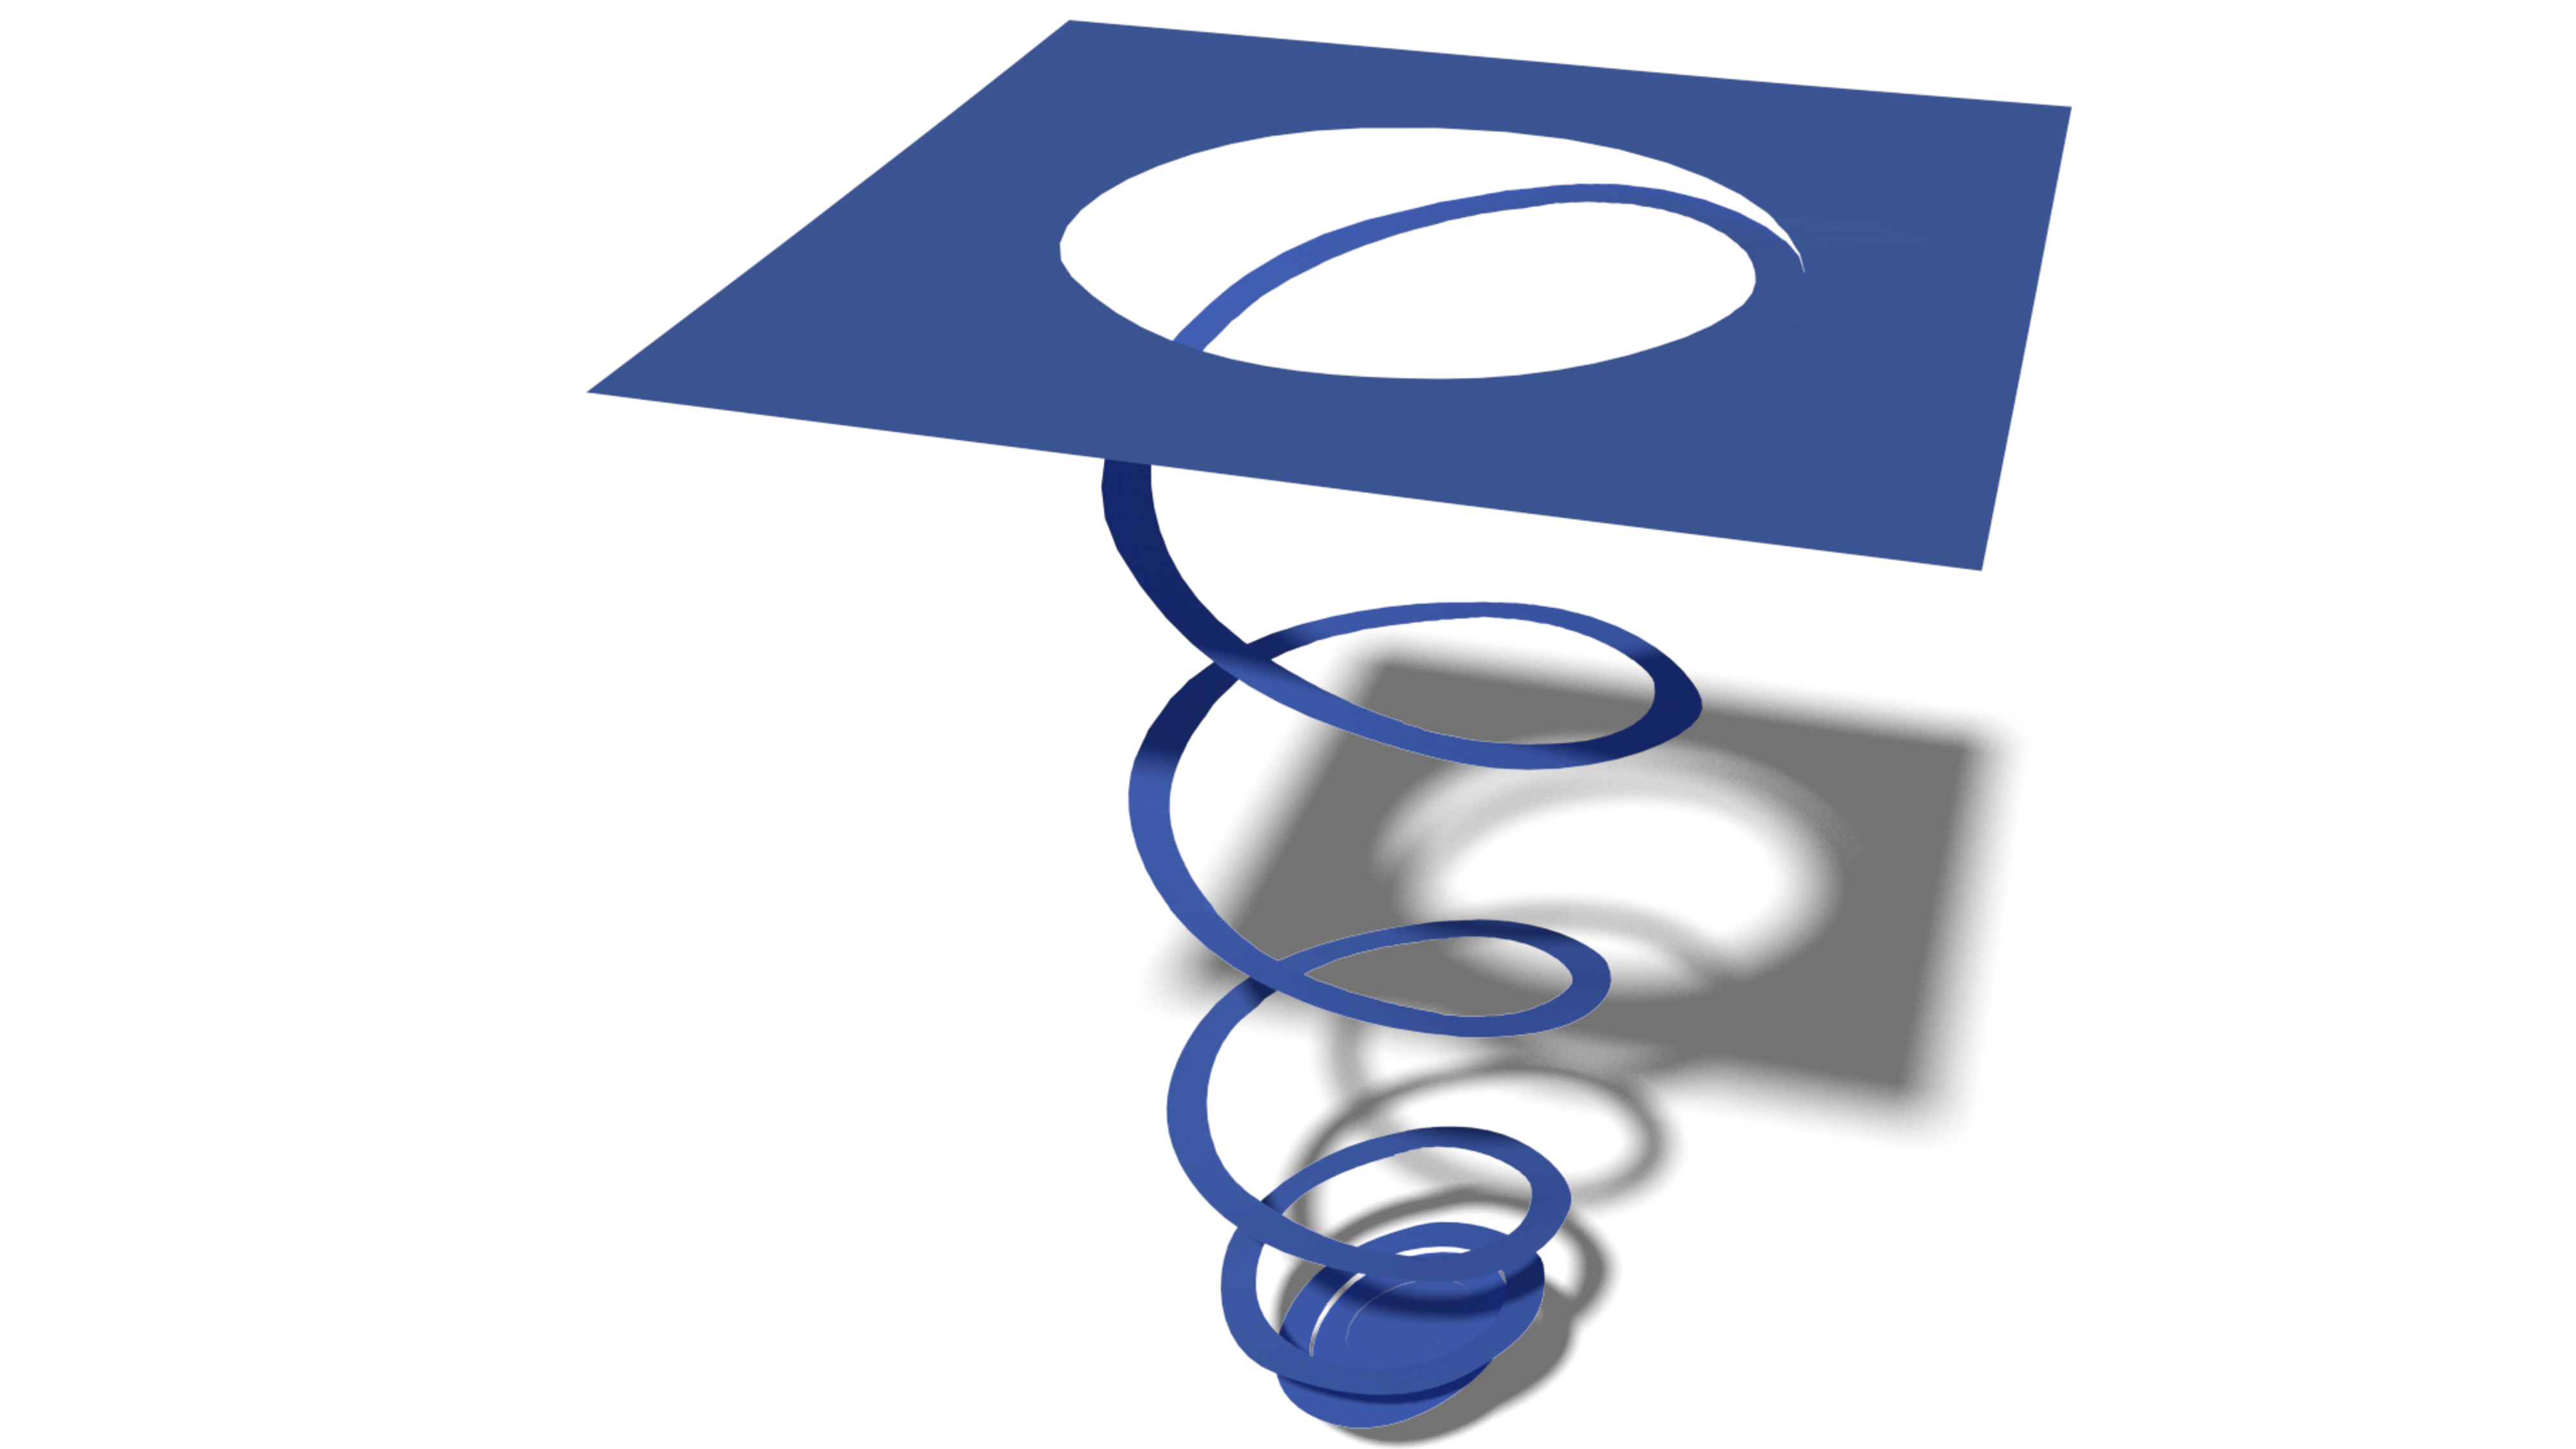
\includegraphics[width=\linewidth]{images/cutting-mig2015/Spiral2.pdf}
		\caption{\label{fig:spiral}}
	\end{subfigure}
	\hfill
	\begin{subfigure}[b]{0.45\linewidth}
		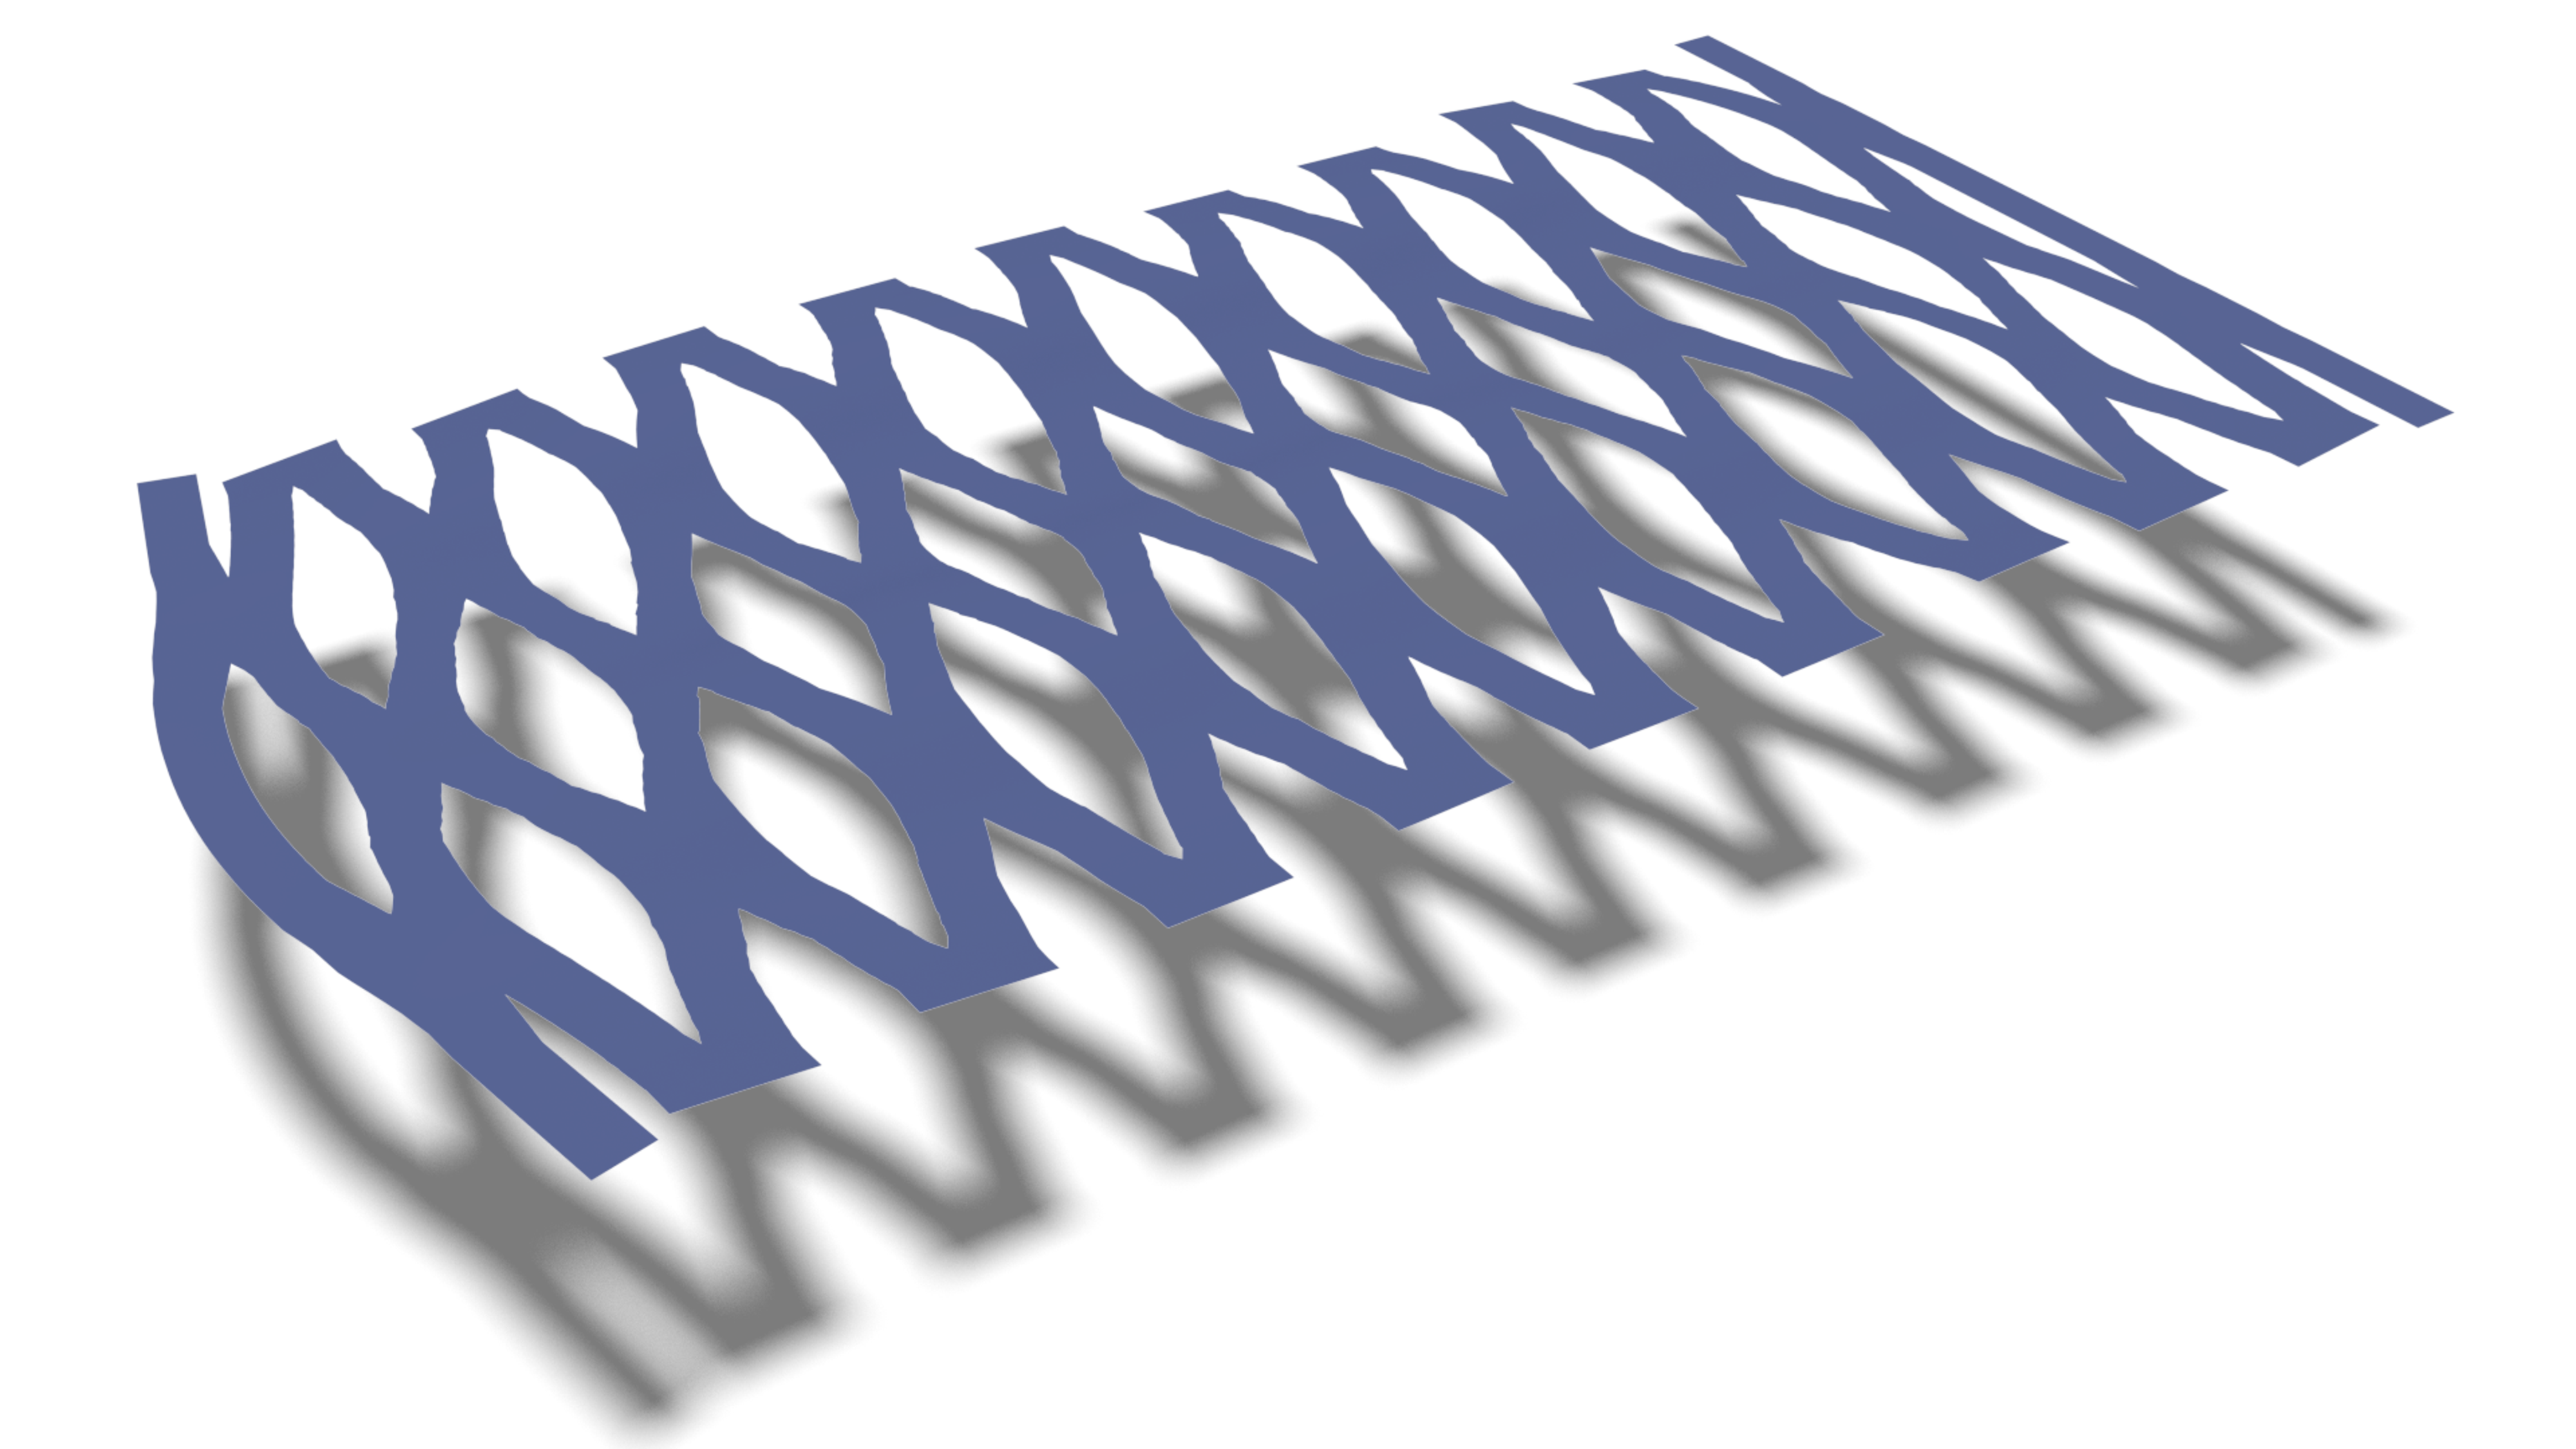
\includegraphics[width=\linewidth]{images/cutting-mig2015/Kirigami.pdf}
		\caption{\label{fig:kirigami}}
	\end{subfigure}
	\caption[Frame-based cutting: Spiral and Kirigami cutting examples]{\label{fig:Cutting_Teaser} Progressive cutting of a spiral using only five control frames (a). Simulating complex deformations resulting from Kirigami cutting (b). Note that an horizontal stretching force results into a twist of the bands of material, as in real experiments using paper.}
\end{figure}

Detailed cuts can be performed and separated components can be handled as shown in Figure \ref{fig:patchwork}. In a cloth sheet, we progressively cut bunny, teapot, dragon and armadillo shapes. Each time a new object is completely cut, it is automatically re-sampled with additional frames.
\paragraph*{}
As we explained, the non-manifold grid can represent an arbitrary number of connectivity in one cell. This is particularly useful in order to represent intersecting cuts as shown in Figure \ref{fig:vortex}.

\begin{figure}[!h]
	\centering
	\begin{subfigure}[b]{0.32\linewidth}
		\centering
		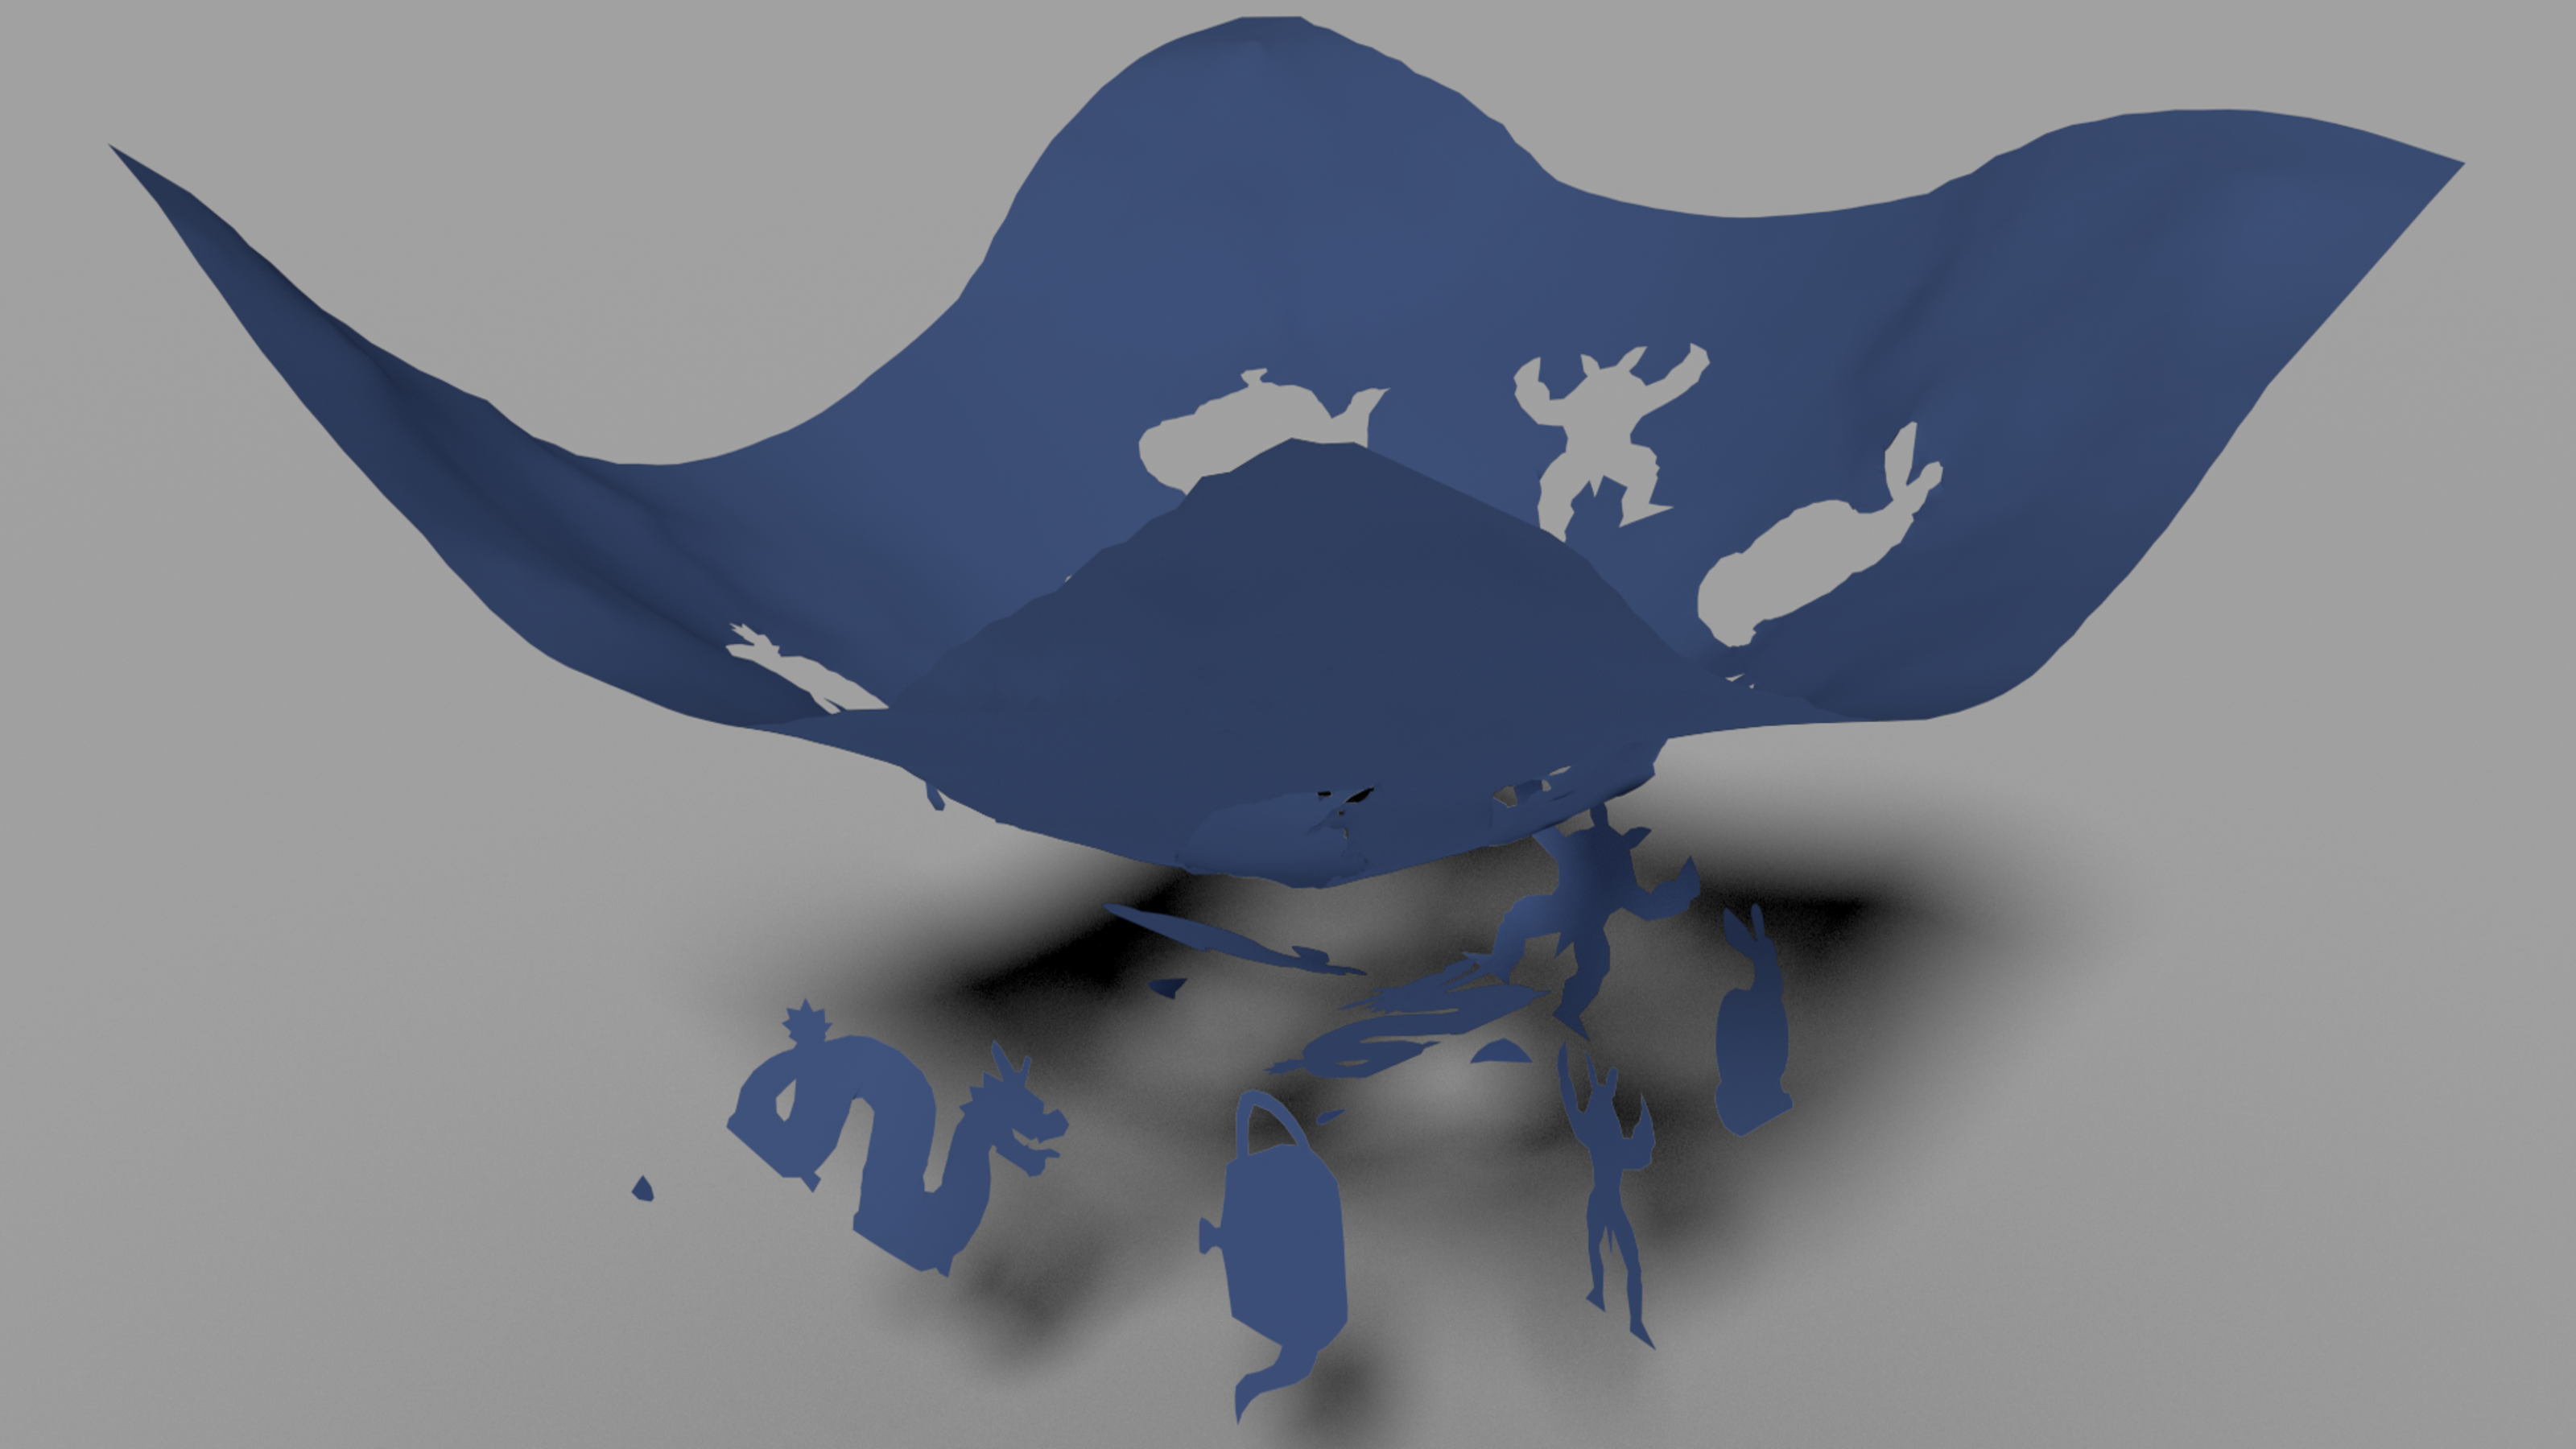
\includegraphics[width=\linewidth]{images/cutting-mig2015/Patchwork.pdf}
		\caption{\label{fig:patchwork}}
	\end{subfigure}
	\hfill
	\begin{subfigure}[b]{0.32\linewidth}
		\centering
		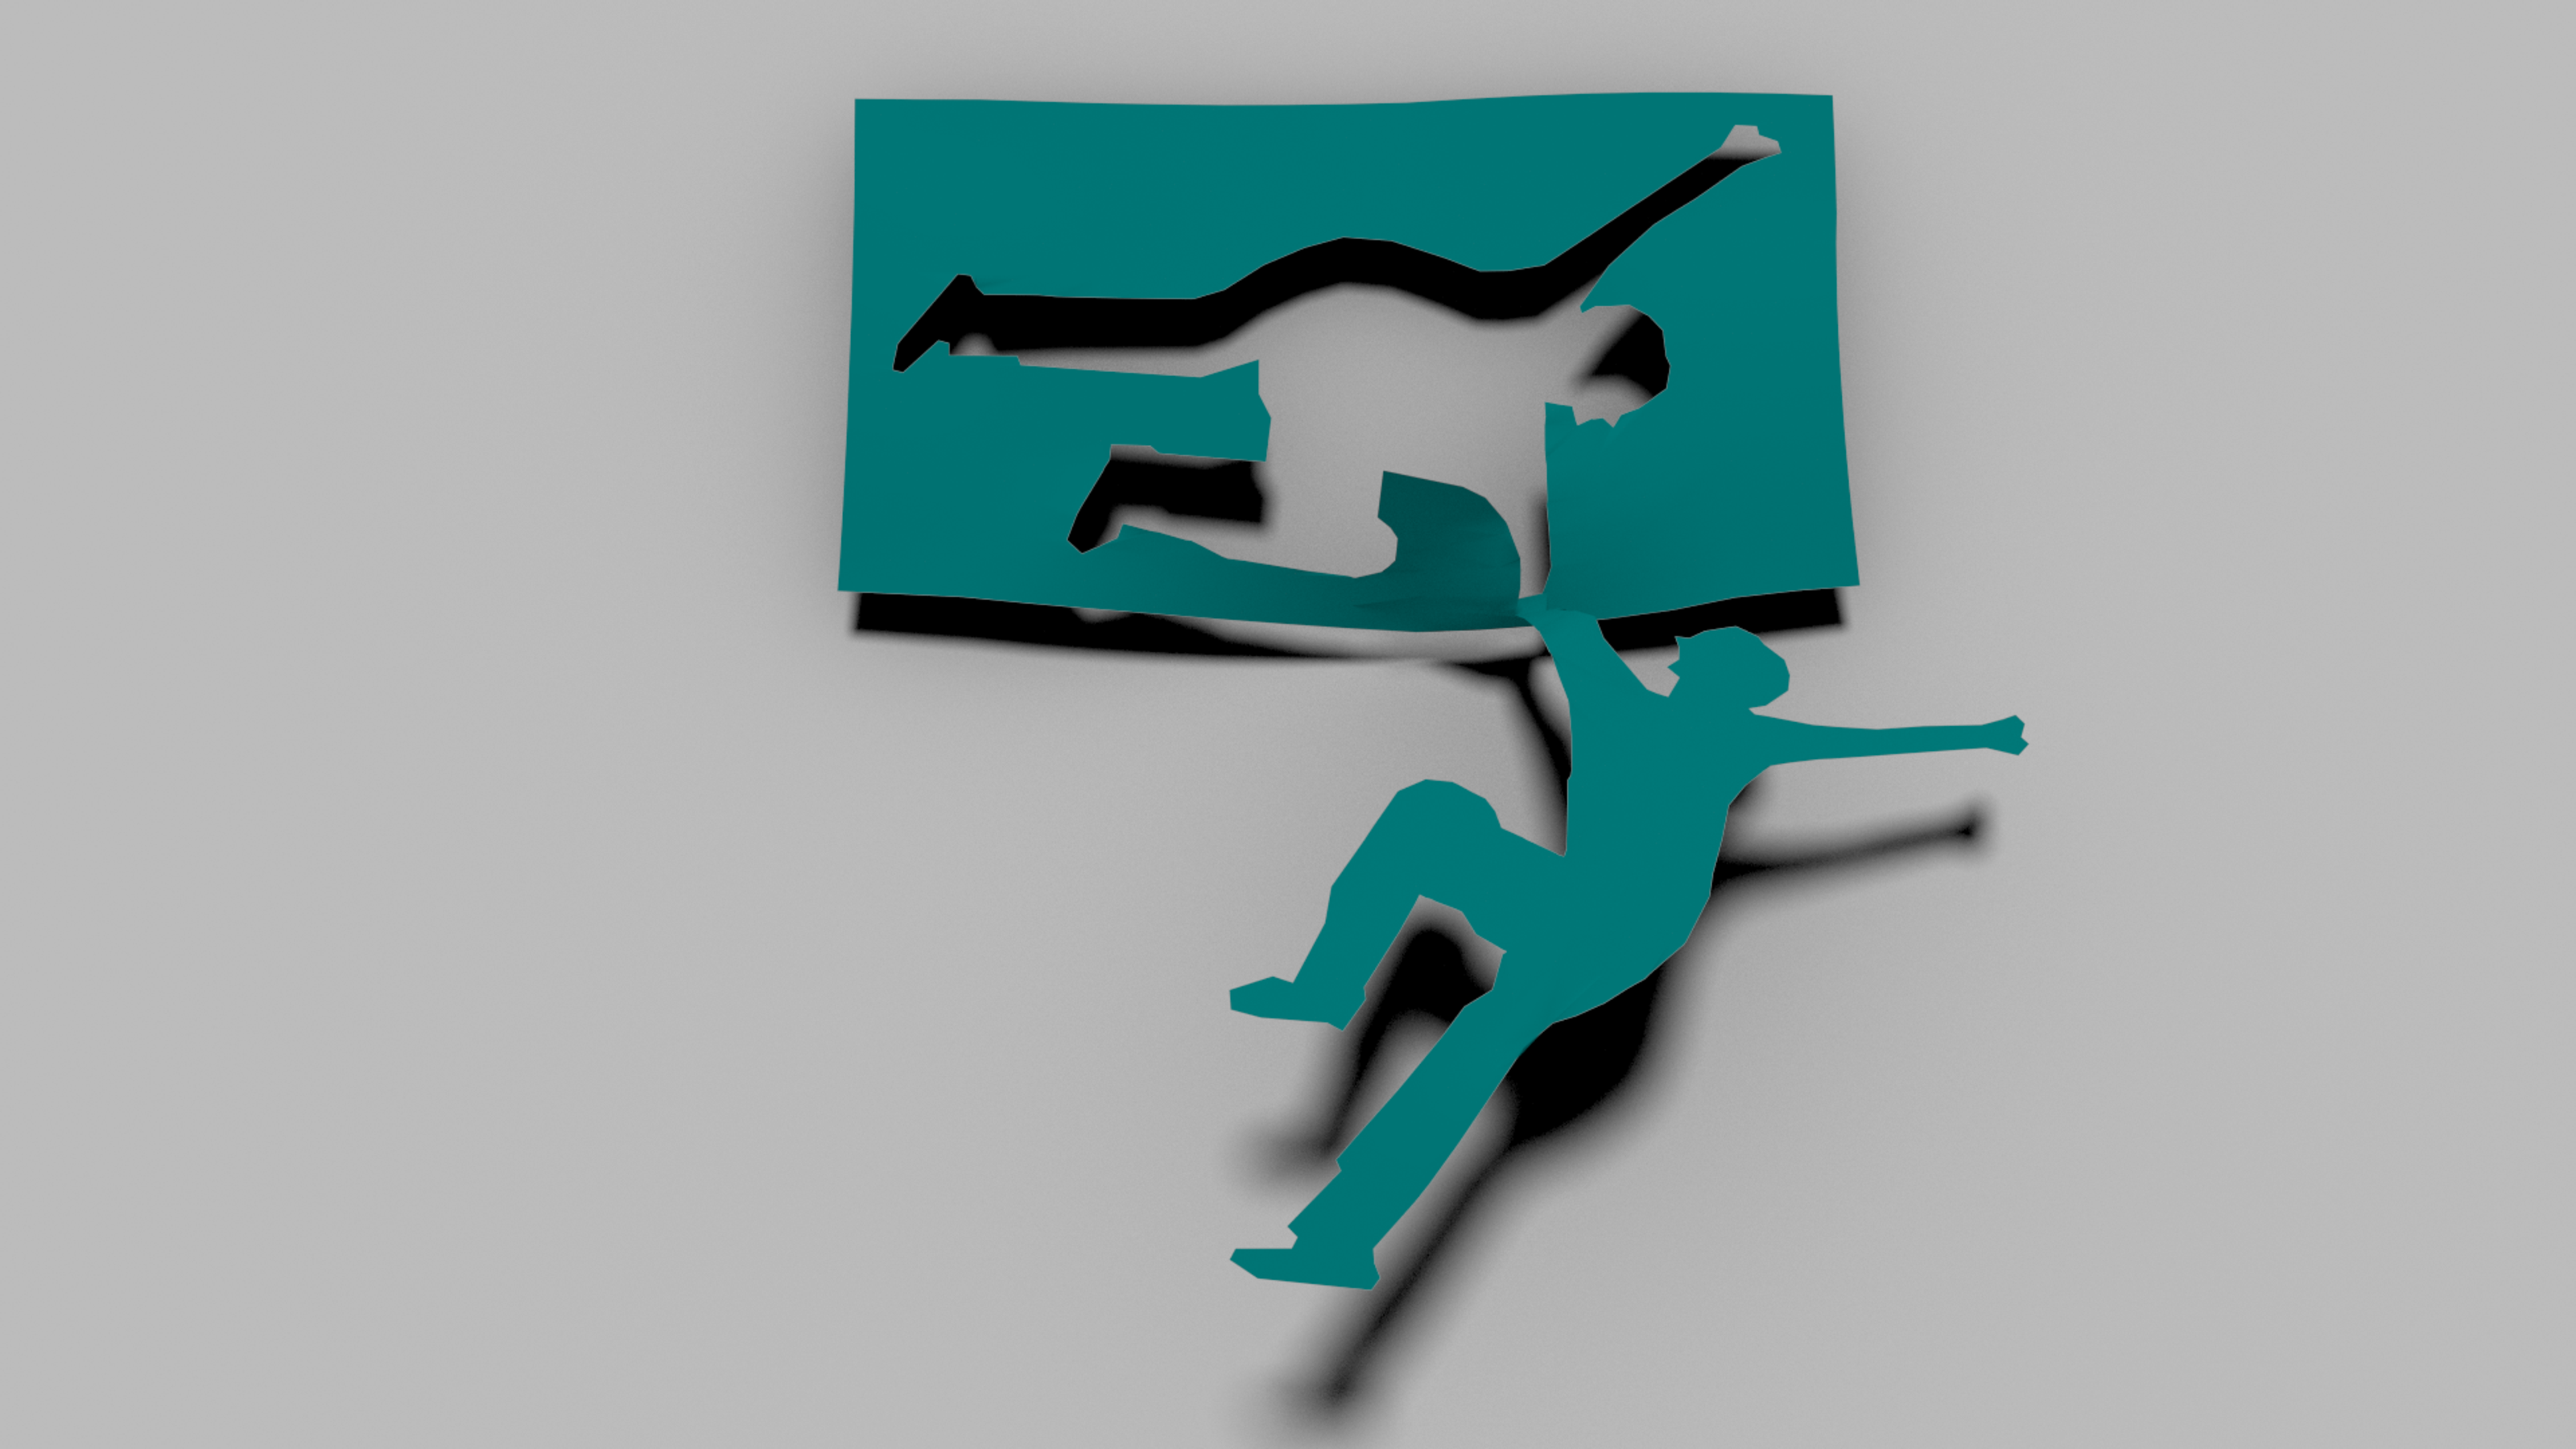
\includegraphics[width=\linewidth]{images/cutting-mig2015/FallingGuy.pdf}
		\caption{\label{fig:fallingguy}}
	\end{subfigure}
	\hfill
	\begin{subfigure}[b]{0.32\linewidth}
		\centering
		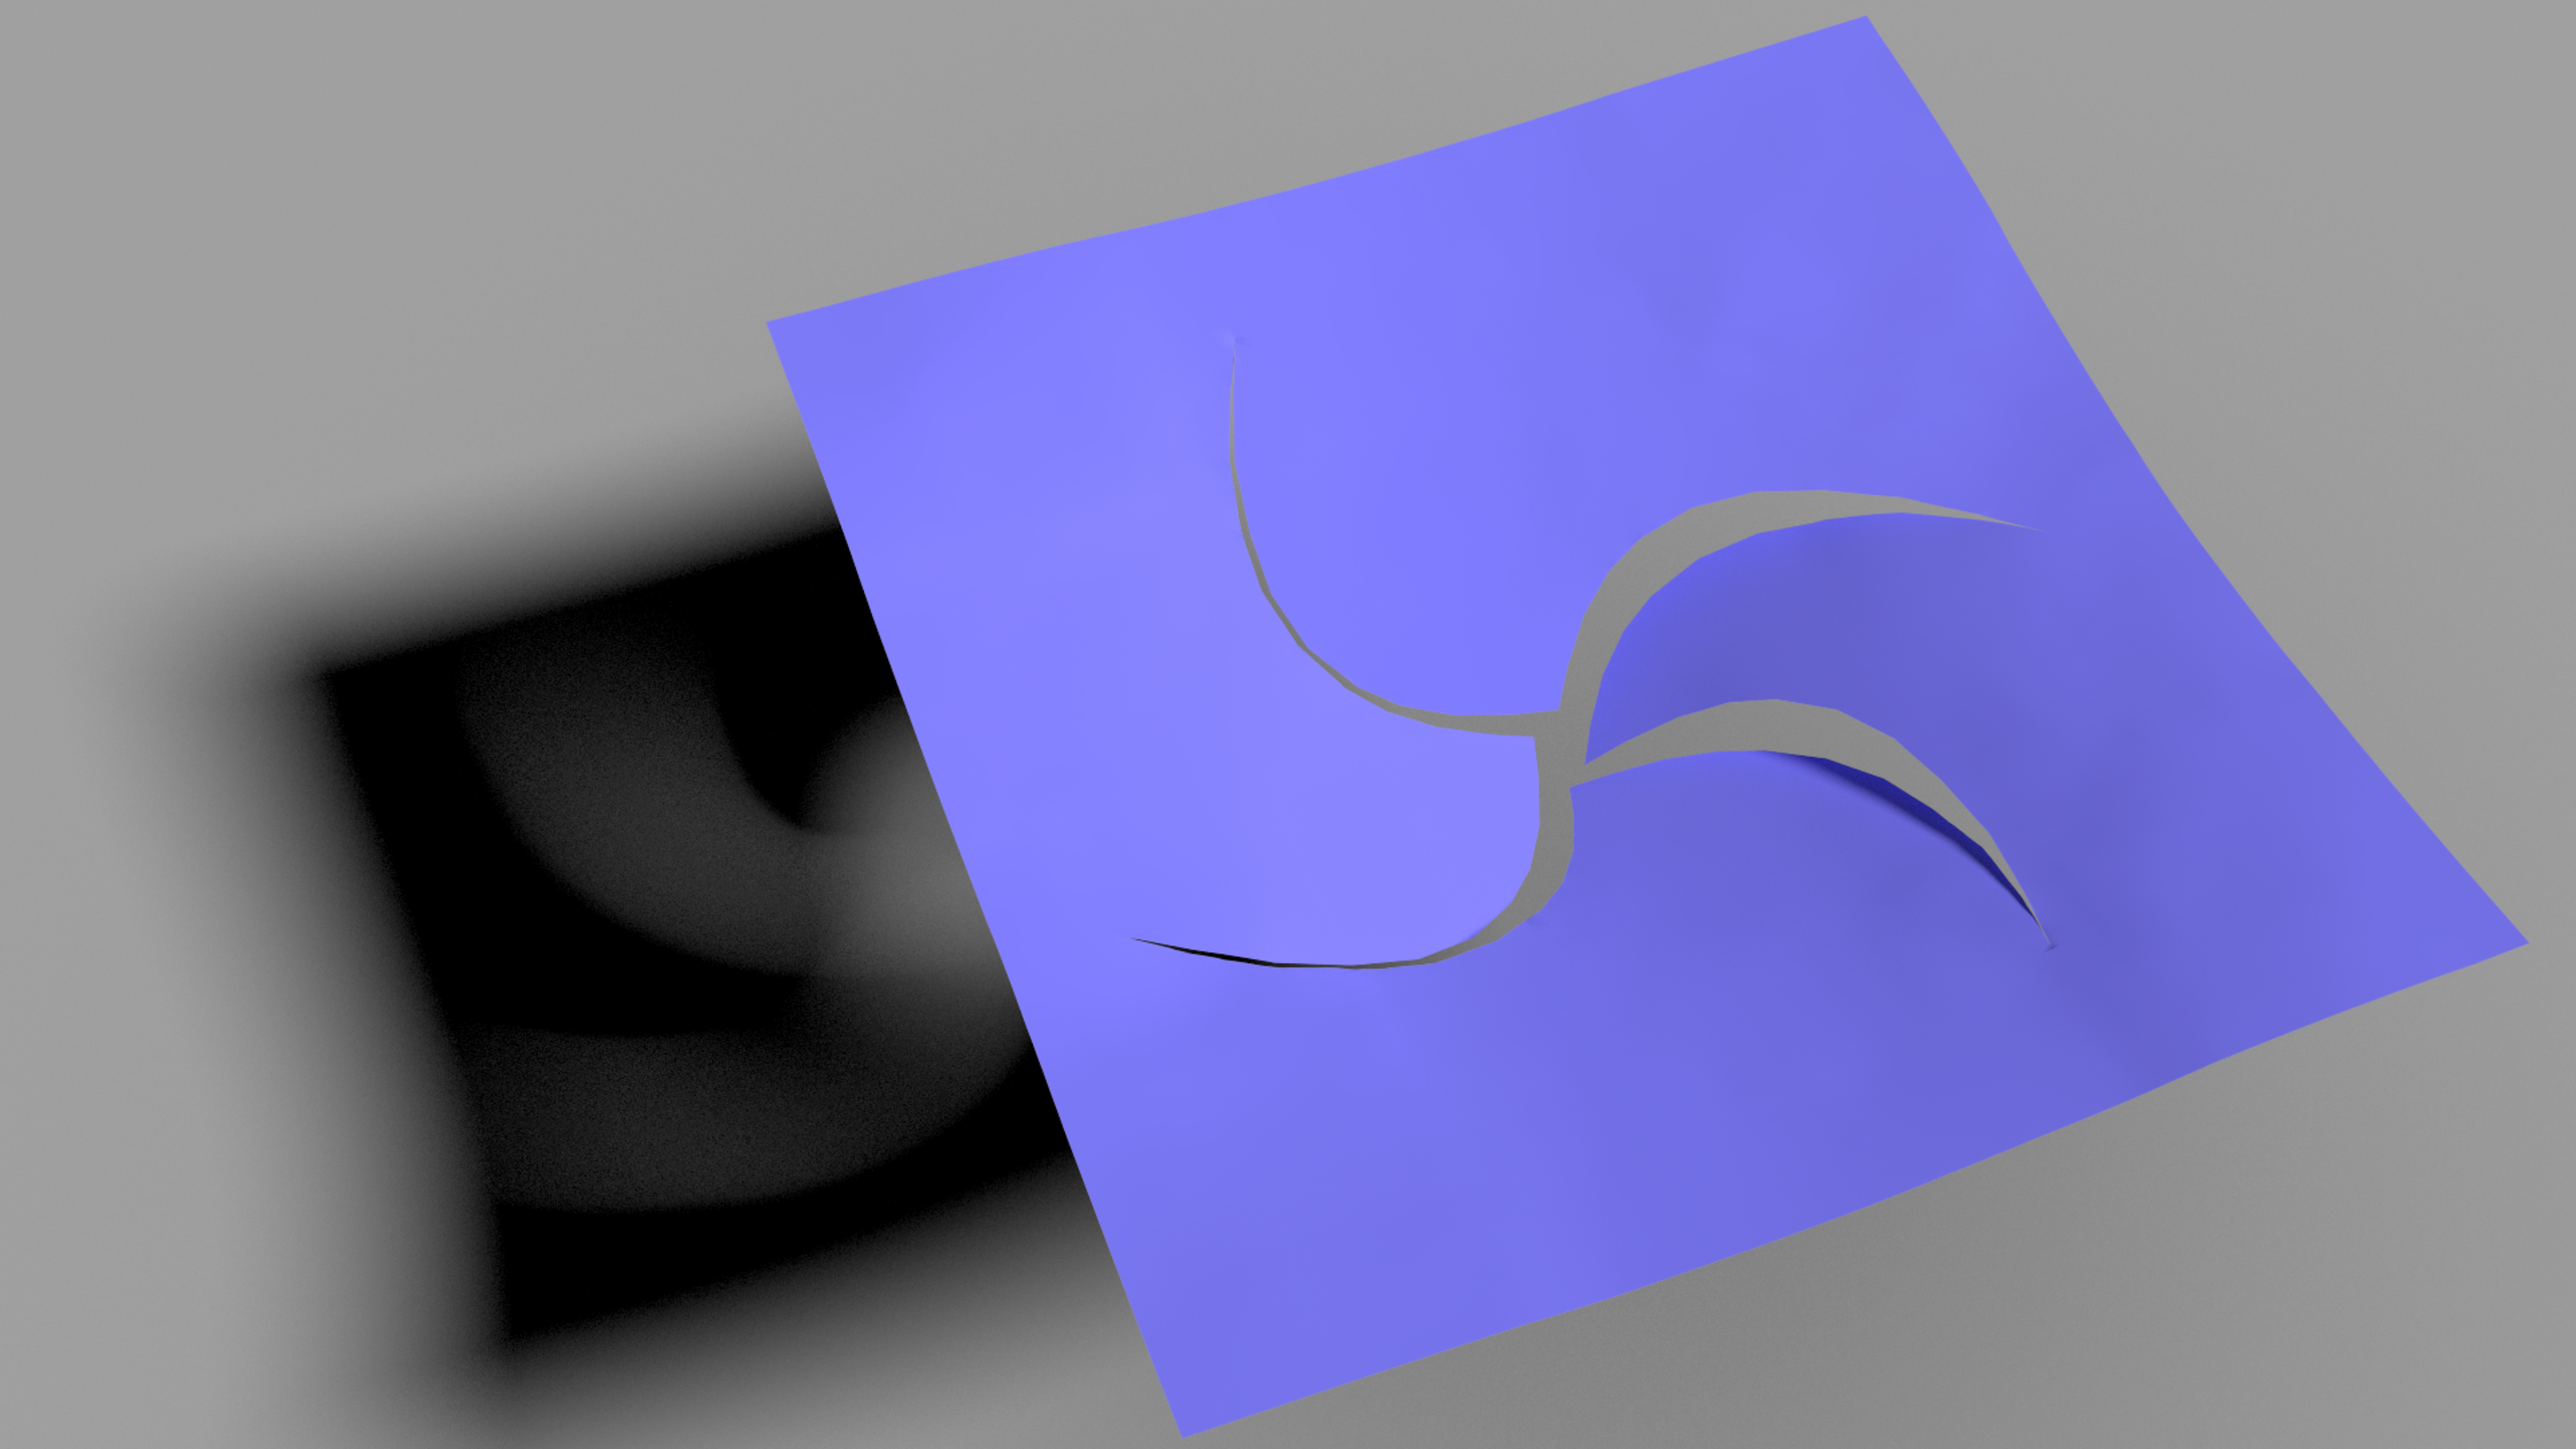
\includegraphics[width=\linewidth]{images/cutting-mig2015/Vortex.pdf}
		\caption{\label{fig:vortex}}
	\end{subfigure}
	\caption[Frame-based cutting: Examples of detailed cutting]{\label{fig:result} (a) Several highly detailed shapes are cut in a deformable sheet. Each disconnected part is automatically re-sampled with additional control frames. (b) Simulation of a highly detailed cut that falls under gravity and remains attached to the main part by a thin piece of paper. (c) Two cuts intersect to form a vortex shape. This illustrates the abilities of the non-manifold grid to handle multiple intersecting cuts.}
\end{figure}

All our examples run at interactive frame rate during the whole simulation (see Table \ref{tab:performance}). Frame rates were collected on a twelve-core 3.20 GHz Intel Xeon CPU with 15.6 GB RAM. 
\addtolength{\tabcolsep}{-1.5pt}
\begin{table}[!h]
	\centering
	\scalebox{0.63}
	{
		\begin{tabular}{l|c|cc|cc|c|c|ccc}
			& & \multicolumn{2}{c|}{\#frame} & \multicolumn{2}{c|}{\#vertices} & & & \multicolumn{3}{c}{Lowest FPS}\\
			Name & Grid Size & Initial & Final & Initial & Final & \#collision & \#integration & \begin{tabular}{c}Before \\ Cutting\end{tabular}  & \begin{tabular}{c}During \\ Cutting\end{tabular}  & \begin{tabular}{c}After \\ Cutting\end{tabular}  \\ \hline
			Spiral (Fig. \ref{fig:spiral}) & $40 \times 40$ & $5$ & $5$ & $81$ & $2111$ & $200$ & $200$ & $60$ & $14.4$ & $60$\\ 
			Kirigami (Fig. \ref{fig:kirigami}) & $68 \times 68$ & $47$ & $47$ & $4225$ & $7453$ & $600$ & $800$ & $11.3$ & $3.2$ & $10.9$\\ 
			Patchwork (Fig. \ref{fig:patchwork}) & $50 \times 50$ & $5$ & $12$ & $4225$ & $8253$ & $200$ & $200$ & $60$ & $6.8$ & $45$\\
			Vortex (Fig. \ref{fig:vortex}) & $68 \times 68$ & $5$ & $5$ & $4225$ & $4889$ & $200$ & $200$ & $45$ & $7.2$ & $35.7$\\
			FallingGuy (Fig. \ref{fig:fallingguy}) & $100 \times 50$ & $10$ & $10$ & $289$ & $861$ & $500$ & $500$ & $60$ & $8.2$ & $60$\\
		\end{tabular}
	}
	\caption[Frame-based cutting: Resolution \& timings]{\label{tab:performance} Resolution of the different components of the simulation and timings.}
\end{table}
\addtolength{\tabcolsep}{1.5pt}

We noticed that even if a cut only concern a few grid cells, the number of data to re-compute is much more important. This comes from the fact that each frame can cover a large region and changes arising from a local cut can be important. Fortunately, our incremental update mechanisms allows to save numerous unnecessary computations as shown in Table \ref{tab:incrementalUpdate}. 

\begin{table}[!h]
	\centering
	\scalebox{0.7}
	{
		\begin{tabular}{l|ccccc}
			& \multicolumn{4}{c}{Percentage of update for a cutting step} \\
			Name & \%grid cell &\%shape function cell & \%vertices & \%collision nodes & \%integration points \\ \hline
			Spiral (Fig. \ref{fig:spiralMesh}) & $0.07$ & $28.1$ & $61.5$ & $27.2$ & $41.3$\\
			Kirigami (Fig. \ref{fig:kirigami}) & $1.06$ & $15.9$ & $17.8$ & $15.8$ & $20.3$\\
			Patchwork (Fig. \ref{fig:patchwork}) & $0.02$ & $2.78$ & $4.33$ & $2.55$ & $7.15$\\
			Vortex (Fig. \ref{fig:vortex}) & $0.08$ & $10.3$ & $12.8$ & $9.2$ & $24.2$\\
			FallingGuy (Fig. \ref{fig:fallingguy}) & $0.09$ & $5.84$ & $11.4$ & $5.77$ & $14.9$\\
		\end{tabular}
	}
	\caption[Frame-based cutting: Incremental update timings]{\label{tab:incrementalUpdate} Percentage of updated data in a cutting time step. We averaged the percentage for the whole cutting time. We notice that even if very few grid cell are affected, it implies important changes on the shape functions and the samples that are associated to these values.}
\end{table}

%%%%%%%%%%%%%%%%%%%%%%%%%%%%%%%%%%%%%%%%%%%%%%%%%%%%%%%%%%%%%%%%
%                      DISCUSSION 
%%%%%%%%%%%%%%%%%%%%%%%%%%%%%%%%%%%%%%%%%%%%%%%%%%%%%%%%%%%%%%%%
\section{Discussion and concluding remarks} 
\label{sec:cutting_conclusion}

In this chapter, we presented a novel method to simulate highly detailed cuts with a sparse set of control nodes which allows interactive frame rates. This approach can be seen as a reduced simulation that handles topological changes without requiring expensive precomputations. Of course, our work is not without limitations and brings interesting directions for future work.

Firstly, as very few frames are used, one cut may generate large changes in the weight distribution and produce popping artifacts that cannot be avoided using our interpolation strategy. This is particularly noticeable when simulating soft materials and can be seen in some of the examples of our accompanying video. Strategies proposed by~\cite{Narain2013} and~\cite{Tournier2014} in the context of adaptive simulations could be used to limit this problem. 

Secondly, for large deformations, the surface can look bumpy. There are several reasons for this problem. Linear blend skinning, used to approximate the displacement field, produces well known artifacts that could be solved using a better skinning approach such as dual quaternion skinning. Also, the shape functions derivatives are discontinuous and this is particularly noticeable during high deformations. One could easily change the shape functions and still use the non-manifold grid to depict the topology.

Thirdly, our implementation is far from being optimal. Currently the non-manifold grid and the shape functions are re-computed from scratch at each cut. We could enjoy a dynamic acceleration structure to incrementally update our non-manifold grid. Shape functions could also be incrementally updated. Finally, there are several parts of our method that could enjoy parallelization such as samples interpolation.

Finally, we would like to extend our work to 3D. The implementation of our current non-manifold grid would require a tetrahedron representation of the object. We would like to investigate the method of~\cite{Remillard2013} to build this structure only from the object surface. We think that the frame-based framework can be used to produce interactive detailed fracture simulation. The main challenge is to accurately compute stress tensors which are then used to determine fracture direction. Instead of using a dense sampling of frames and integration points to compute the stress tensors, we would like to combine a low resolution stress tensor measurement with procedural detail generation as in the work of~\cite{Chen2014} and~\cite{Lejemble2015}. In a similar direction, we would like to investigate advanced sampling strategies in order to automatically determine how many frames are required for a given region. This would involve the material property, the size and the shape of the region that needs to be sampled.
\paragraph*{}
In this chapter and the previous one, we explored different simulation techniques which enables efficient computations and topological changes. 
When experimenting these two methods, a substantial amount of time was dedicated to adjust the parameters of the simulation: time step, damping, stiffness, initial and boundary conditions, in order to achieve the results we had in mind.
As we explained in Section~\ref{sec:starSimulationControl}, controlling a physics-based simulation is a hard problem, especially when it exhibits complex topological changes, such as in liquid simulations.
In the next chapter, we address this problem by proposing a novel method to sculpt liquids animations using intuitive tools inspired from shape modeling.
